\chapter{Strumenti Utilizzati}
L'applicativo software sviluppato per eseguire benchmark di algoritmi per l'image processing fornisce un ambiente standardizzato per eseguire una serie di test e misurare le prestazioni in modo oggettivo.\par
Per lo sviluppo di tale applicativo si è fatto affidamento a svariate tecnologie e librerie esterne.

{\section{Python}

\begin{wrapfigure}{r}{0.20\textwidth}
	\centering
	
\includegraphics[scale=0.1]{python-logo}
\end{wrapfigure}
\textit{Python} è un \textit{linguaggio di programmazione ad alto livello} con una sintassi semplice e intuitiva. È un linguaggio interpretato con tipizzazione dinamica debole, ovvero la tipizzazione delle variabili avviene durante l'esecuzione del codice. Questo rende Python molto flessibile e facile da utilizzare.\par
Lo sviluppo di Python ha avuto inizio negli anni '90 da Guido van Rossum e si è rapidamente affermato come uno dei linguaggi di programmazione più popolari, grazie sopratutto alla sua versatilità in svariate campi, tra cui web development, sviluppo di software scientifico, automazione, machine learning, statistica e molto altro ancora.\par
Uno dei punti di forza di Python è la sua estesa libreria standard, che include molte funzioni già implementate per molte attività comuni, come l'elaborazione di stringhe, la gestione dei file, la connessione a database, il parsing di XML e JSON. Ad affiancare la libreria standard ci sono anche numerosi sviluppatori che hanno creato molti framework e librerie esterne per molte applicazioni specifiche.\par
In sintesi, Python è un linguaggio di programmazione estremamente potente e versatile che rende facile sviluppare software in molti ambiti diversi. La sua sintassi semplice e intuitiva, la vasta libreria standard e la forte comunità di sviluppatori lo rendono una scelta popolare per molti programmatori.

\subsection{Ragioni di preferenza}
Nonostante Python non sia un linguaggio orientato alle performance, come ad esempio C++, la decisione dell'utilizzo ricade sulla semplicità e flessibilità delle funzionalità del linguaggio. Ciò ha permesso uno sviluppo veloce e nei limiti tempistici dello studente.

Il software non ha applicazioni pratiche bensì puramente accademici, in quanto la maggior parte delle librerie per image processing fa uso di \textit{binding} verso i linguaggi più performanti come C++.

{\section{Tkinter}
	
	\begin{wrapfigure}{l}{0.20\textwidth}
		\centering
		
\includegraphics[scale=0.30]{tkinter}
	\end{wrapfigure}
\textit{Tkinter} è una \textit{libreria di interfaccia grafica} (GUI) per Python. Consente agli sviluppatori di creare applicazioni con una grafica interattiva utilizzando un set di \textit{widget} basati sul toolkit \textit{Tcl/tk}. Tkinter è inclusa nella libreria standard di Python, quindi non richiede installazioni aggiuntive, ciò lo rende altamente portabile e può essere eseguito su diverse piattaforme come Windows, macOS e Linux senza necessità di scrivere codice specifico per una piattaforma.

Tkinter offre una vasta gamma di widget predefiniti, come pulsanti, caselle di testo, etichette, menu, finestre di dialogo e molti altri, che semplificano la creazione di interfacce utente. I widget possono essere posizionati e organizzati in frame utilizzando metodi di layout come \textit{pack()}, \textit{grid()} o \textit{place()}, che richiamano rispettivamente layout \textit{assoluto, a griglia o fluido}.

Un ulteriore punto di forza di Tkinter è la sua integrazione con altri strumenti e librerie di Python, come ad esempio con la popolare libreria \textit{Matplotlib} per visualizzare grafici o con la libreria \textit{Pillow (o PIL)} per visualizzare all'interno di un'applicazione Tkinter.

In conclusione, Tkinter è una libreria versatile e potente per lo sviluppo di interfacce grafiche in Python. La sua facilità d'uso, la portabilità, la flessibilità di progettazione, l'integrazione con altri strumenti e il supporto della comunità la rendono una scelta popolare per creare applicazioni con una grafica interattiva.
	
\subsection{CustomTkinter}
Nonostante Tkinter offra anche opzioni per la personalizzazione dell'aspetto dei widget con cui si possono definire stili, colori, dimensioni dei caratteri e altre proprietà per creare interfacce utente attraenti con facilità, per lo sviluppo dell'applicativo si è preferito utilizzare la libreria \textit{CustomTkinter} sviluppato dall'utente GitHub \textit{TomSchimansky}.

CustomTkinter è una libreria GUI per Python basata su Tkinter. Offre nuovi e moderni widget, completamente personalizzabili. Tali widget possono essere creati ed utilizzati analogamente ai widget predefiniti di Tkinter, possono anche essere utilizzati in combinazione con i widget di quest'ultimo. I widget e il \textit{color-scheme} delle finestre si adattano all'aspetto del sistema in cui viene eseguito, ma è anche possibile impostare manualmente la modalità \textit{chiaro} o \textit{scuro}.

CustomTkinter supporta la scalatura HighDPI, permettendo di avere un aspetto coerente e moderno anche su sistemi ad alta risoluzione.

{\section{Pillow}
	
	\begin{wrapfigure}{r}{0.20\textwidth}
		\centering
		
\includegraphics[scale=0.3]{pillow}
	\end{wrapfigure}
	\textit{Pillow} è una libreria Python per l'elaborazione delle immagini, sviluppata come fork di \textit{PIL} (\textit{Python Imaging Library}). Grazie alla sua vasta gamma di funzionalità è diventata la libreria di facto per lavorare con immagini in Python.
	
	La libreria fornisce un'interfaccia supporta immagini in diversi formati, tra cui JPEG, PNG, BMP, TIFF e molti altri. Può facilmente aprire un'immagine da file o sequenza binaria, modificarla, applicare filtri, ridimensionarla, ritagliarla, aggiungere testo e molto altro ancora.
	
	Offre un'ampia gamma di metodi e funzioni per eseguire operazioni di manipolazione delle immagini: è possibile accedere ai singoli pixel dell'immagine, modificarli direttamente o utilizzare funzioni predefinite e ottimizzate per applicare effetti e trasformazioni tramite l'utilizzo dell'interfaccia \textit{ImageFilter}.
	
	In conclusione, Pillow è anche compatibile con NumPy, una libreria molto diffusa per il calcolo scientifico in Python. Questa integrazione consente di convertire agevolmente le immagini Pillow in array NumPy e viceversa, aprendo così la strada a numerose possibilità di elaborazione delle immagini utilizzando strumenti matematici avanzati.

{\section{NumPy}
	
	\begin{wrapfigure}{l}{0.20\textwidth}
		\centering
		
\includegraphics[scale=0.30]{numpy}
	\end{wrapfigure}
	\textit{NumPy} è una libreria Python ampiamente utilizzata per il \textit{calcolo scientifico e numerico}. Offre un potente oggetto array multidimensionale chiamato \textit{ndarray}, che consente di gestire grandi quantità di dati in modo efficiente.
	
	Permette di eseguire \textit{operazioni matematiche e algebriche su array}, come addizione, sottrazione, moltiplicazione e divisione, sia tra singoli elementi che tra interi array. Tali operazioni vengono eseguite in modo vettoriale, ovvero vengono applicate simultaneamente a tutti gli elementi dell'array, rendendo il calcolo molto efficiente.
	
	Oltre alle operazioni di base, NumPy offre anche una vasta gamma di \textit{funzioni matematiche avanzate}, come funzioni trigonometriche, esponenziali, logaritmiche e statistiche. 
	
	L'efficienza di NumPy è dovuta al fatto che gli array NumPy sono implementati in linguaggio C, il che consente di sfruttare al massimo la velocità di esecuzione.
	
	Complessivamente, NumPy è uno strumento fondamentale per il calcolo scientifico e numerico in Python, offrendo un'implementazione efficiente di array multidimensionali e una vasta gamma di funzioni matematiche.
	
\subsection{Restrizioni nell'utilizzo}
Per evitare uno sbilanciamento dei risultati, causato dall'implementazione in C degli ndarray, all'interno del progetto l'utilizzo della libreria NumPy è stato limitato alle \textit{attività di minor rilievo} come ad esempio la generazione di un kernel Gaussiano o ricerca all'interno di matrici. 
	
{\section{Matplotlib}
	
	\begin{wrapfigure}{r}{0.20\textwidth}
		\centering
		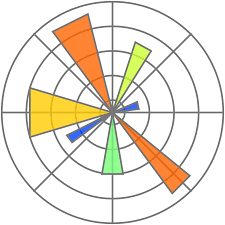
\includegraphics[scale=0.3]{matplotlib}
	\end{wrapfigure}
\textit{Matplotlib} è una libreria Python ampiamente utilizzata per la \textit{visualizzazione di dati e la creazione di grafici}. Fornisce un'interfaccia intuitiva per creare una vasta gamma di \textit{grafici}, inclusi \textit{grafici a linee}, \textit{grafici a dispersione}, \textit{istogrammi}, \textit{grafici a barre}, \textit{grafici a torta} e molti altri.

Permette di personalizzare svariati aspetti dei grafici, come colori, stili di linea, etichette degli assi e titoli.

Un punto di forza della libreria è la sua integrazione con NumPy, precedentemente introdotta. È possibile utilizzare gli array NumPy come dati di input per generare grafici, semplificando notevolmente il processo di visualizzazione dei dati.

In conclusione, Matplotlib è una potente libreria di visualizzazione dei dati in Python, la cui flessibilità, facilità d'uso e integrazione con NumPy la rendono uno strumento essenziale per gli scienziati, gli ingegneri e i data scientist.
\newpage
{\section{GIL e Multiprocessing}
	
	\begin{wrapfigure}{l}{0.20\textwidth}
		\centering
		
\includegraphics[scale=0.30]{multiprocessing}
	\end{wrapfigure}
Il \textit{GIL (Global Interpreter Lock)} è un meccanismo di gestione dei thread utilizzato nell'implementazione standard di CPython, l'interprete di Python di riferimento, allo scopo di consentire un'interazione più sicura con gli oggetti Python.

Il GIL è un \textit{vincolo} che permette a solo un thread alla volta di eseguire istruzioni Python, \textbf{anche su sistemi con processori multi-core}. Questo significa che, nonostante si possano utilizzare thread multipli, essi non possono eseguire istruzioni simultaneamente: quando un thread acquisisce il GIL, gli altri thread devono attendere il loro turno per eseguire codice Python.

Rappresenta un \textit{limite sulle prestazioni} in alcune situazioni specifiche, in particolare quando si tenta di applicare una parallelizzazione al fine di sfruttare appieno le capacità di elaborazione parallela di un sistema multi-core.

Il modulo \textit{multiprocessing}, incluso nelle librerie standard di Python, offre una soluzione per superare le limitazioni del GIL. Fornisce un'interfaccia per la \textit{creazione di processi multipli}, che possono eseguire codice Python \textbf{in modo indipendente} e sfruttare i vantaggi del parallelismo effettivo su sistemi multi-core.

Utilizzando multiprocessing, è possibile suddividere un compito in più processi che vengono essere eseguiti in parallelo. Tali processi comunicano tra loro attraverso la condivisione di dati o l'invio di messaggi tramite code o pipe.

Tuttavia, l'utilizzo di multiprocessing non è privo di svantaggi:
\begin{itemize}
	\item Se il lavoro da eseguire in ogni processo è relativamente semplice e richiede poco tempo di calcolo, il costo aggiuntivo di creare e gestire i processi potrebbe superare i benefici del parallelismo;
	\item Se i processi devono comunicare o dipendere l'uno dall'altro in modo significativo durante l'esecuzione, l'utilizzo di multiprocessing può introdurre complessità aggiuntiva;
	\item Ogni processo creato con multiprocessing ha il proprio spazio di memoria separato. Se il processo richiede una grande quantità di dati da elaborare e mantenere in memoria, l'utilizzo di processi multipli può portare a un consumo eccessivo di memoria;
	\item L'invio di dati tra processi richiede la \textit{serializzazione} e la \textit{deserializzazione} degli oggetti utilizzando \textit{pickle}. Questa conversione non supporta tutti i tipi di dati e introduce un certo overhead, soprattutto per oggetti complessi o di grandi dimensioni;
\end{itemize}